\section{Sagemath là gì?}

SageMath (viết tắt là Sage) là một phần mềm mã nguồn mở được thiết kế nhằm hỗ trợ các phép toán toán học từ cơ bản đến nâng cao. Sage được phát triển bởi giáo sư William Stein tại Đại học Washington vào năm 2005, với mục tiêu tạo ra một công cụ toán học mạnh mẽ nhưng hoàn toàn miễn phí, tương đương với các phần mềm thương mại như Mathematica, Maple, và MATLAB.

\begin{figure}[H]
	\centering
	
\includegraphics[width=0.7\linewidth]{images/screenshot005}
	\caption{Logo phần mềm SageMath phiên bản 10.5}
	\label{fig:screenshot005}
\end{figure}

\subsection{Ý tưởng và động lực phát triển}

\begin{figure}
	\centering
	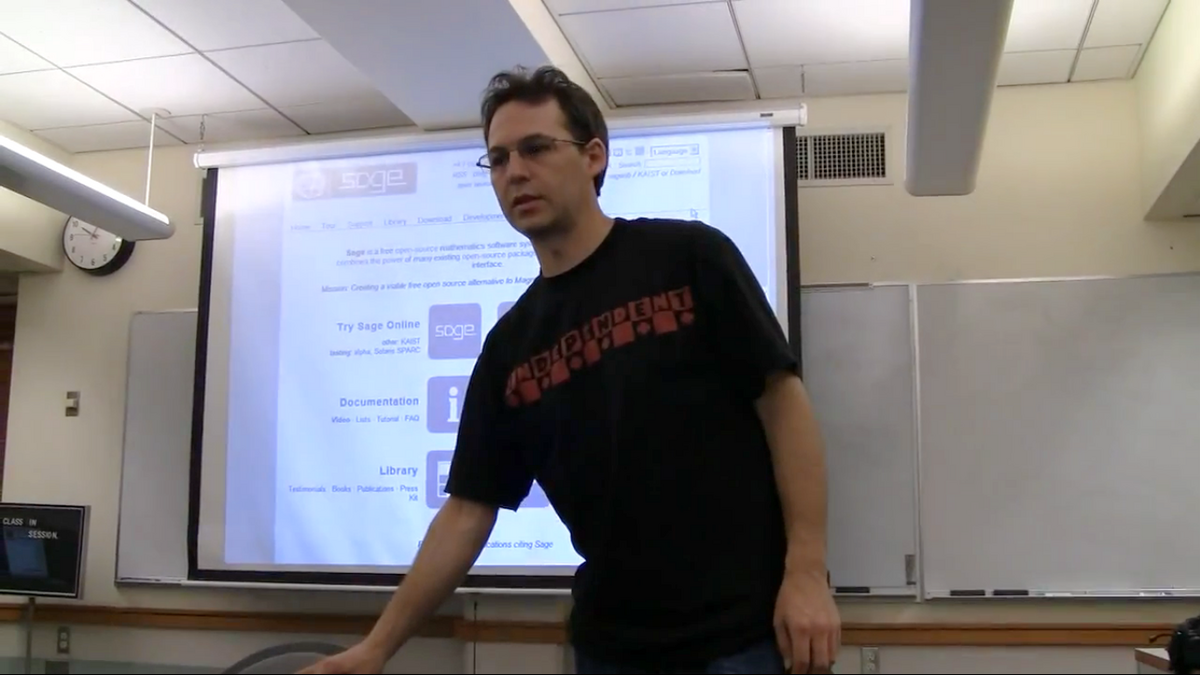
\includegraphics[width=0.7\linewidth]{images/screenshot006}
	\caption{William A. Stein đang nói chuyện về Sage tại REU Toán học năm 2011 tại Đại học Washington}
	\label{fig:screenshot006}
\end{figure}

William Stein, một nhà toán học chuyên về lý thuyết số, nhận thấy rằng các công cụ toán học mạnh mẽ hiện có đều yêu cầu chi phí cao và không thân thiện với người dùng trong cộng đồng nghiên cứu toán học. Với tư duy mã nguồn mở, ông đã quyết định xây dựng một nền tảng kết hợp từ nhiều công cụ toán học hiện có như:
\begin{itemize}
	\item \textbf{Maxima:} Hỗ trợ tính toán đại số trừu tượng.
	\item \textbf{NumPy và SciPy:} Tính toán số học và khoa học.
	\item \textbf{SymPy:} Tính toán trừu tượng.
	\item \textbf{R:} Phân tích thống kê.
	\item \textbf{Matplotlib:} Vẽ đồ thị và trực quan hóa.
\end{itemize}

\subsection{Quá trình phát triển}

Phiên bản đầu tiên của Sage được phát hành vào tháng 2 năm 2005 với tên gọi là "SAGE" (System for Algebra and Geometry Experimentation). Qua nhiều năm phát triển, Sage đã trở thành một hệ thống toán học hoàn chỉnh với khả năng tích hợp nhiều thư viện mạnh mẽ từ cộng đồng Python và các dự án mã nguồn mở khác.

Một cột mốc đáng chú ý trong lịch sử Sage là khi nó chuyển sang tên gọi chính thức là "SageMath" để nhấn mạnh vai trò là một hệ thống tính toán toán học. SageMath được sử dụng rộng rãi trong giảng dạy, nghiên cứu và công nghiệp nhờ tính linh hoạt và miễn phí của nó.

\subsection{Tính mã nguồn mở}

SageMath được phát triển dưới giấy phép GPL (GNU General Public License), nghĩa là bất kỳ ai cũng có thể sử dụng, sửa đổi và phân phối lại phần mềm. Điều này tạo ra một cộng đồng người dùng và phát triển lớn mạnh, với sự tham gia của nhiều nhà nghiên cứu và lập trình viên từ khắp nơi trên thế giới.

\subsection{Những cột mốc quan trọng}

\begin{itemize}
	\item \textbf{2005:} Phát hành phiên bản đầu tiên của SageMath.
	\item \textbf{2007:} SageMath giành giải thưởng FSF (Free Software Foundation) cho dự án phần mềm tự do.
	\item \textbf{2013:} Ra mắt CoCalc (trước đây là SageMathCloud), cho phép sử dụng SageMath trực tuyến.
	\item \textbf{2020:} SageMath được tích hợp hoàn chỉnh với Jupyter Notebook, tạo thuận lợi cho việc sử dụng trong môi trường tính toán khoa học.
\end{itemize}

\subsection{Tầm nhìn và tương lai}

Mục tiêu dài hạn của SageMath là trở thành một hệ thống tính toán toán học mạnh mẽ, thân thiện với người dùng và hoàn toàn miễn phí. SageMath đang tiếp tục được phát triển và hoàn thiện bởi cộng đồng mã nguồn mở, nhằm mở rộng hơn nữa khả năng tính toán và ứng dụng trong nhiều lĩnh vực khoa học, giáo dục và công nghiệp.

\section{So sánh SageMath với các phần mềm Toán học khác}
\begin{table}[H]
	\centering
	\begin{tabularx}{\textwidth}{|X|X|X|X|}
		\hline
		\textbf{Tiêu chí} & \textbf{SageMath} & \textbf{Mathematica / Maple} & \textbf{MATLAB} \\ \hline
		Mã nguồn & Mở hoàn toàn & Đóng & Đóng \\ \hline
		Ngôn ngữ lập trình & Python & Ngôn ngữ riêng biệt & MATLAB \\ \hline
		Tính toán trừu tượng (Symbolic) & Có (qua SymPy, Maxima) & Rất mạnh & Yếu \\ \hline
		Tính toán số & Mạnh (qua NumPy, SciPy) & Có & Rất mạnh \\ \hline
		Tính linh hoạt & Cao nhờ tích hợp nhiều thư viện & Trung bình & Trung bình \\ \hline
		Khả năng mở rộng & Dễ dàng thông qua thư viện Python & Hạn chế & Có nhưng không đa dạng như Python \\ \hline
		Chi phí sử dụng & Miễn phí & Trả phí cao & Trả phí cao \\ \hline
	\end{tabularx}
	\caption{So sánh SageMath với một số phần mềm toán học khác}
\end{table}

SageMath nổi bật nhờ khả năng tích hợp các thư viện hiện đại và tận dụng cộng đồng mã nguồn mở để phát triển liên tục.

\section{Hướng dẫn cài đặt SageMath}

\subsection*{Cài đặt trên Windows}

\begin{itemize}
	\item Truy cập trang chính thức: \texttt{https://www.sagemath.org/download.html}
	\item Tải bản cài đặt phù hợp với hệ điều hành.
	\item Cài đặt như một phần mềm thông thường.
	\item Đối với người dùng nâng cao, có thể sử dụng Windows Subsystem for Linux (WSL) để cài Sage trên Ubuntu.
\end{itemize}

\subsection*{Cài đặt trên Linux (Ubuntu)}

\begin{lstlisting}[language=bash]
	sudo apt update
	sudo apt install sagemath
\end{lstlisting}

\subsection*{Cài đặt trên macOS}

Có thể sử dụng Homebrew:

\begin{lstlisting}[language=bash]
	brew install --cask sagemath
\end{lstlisting}

\section{Sử dụng SageMath trực tuyến không cần cài đặt}

Trong trường hợp người dùng không muốn cài đặt SageMath trực tiếp trên máy tính, có thể sử dụng các nền tảng trực tuyến để chạy các mã SageMath mà không cần cấu hình phức tạp.

\subsection{CoCalc - Collaborative Calculation}

CoCalc (trước đây là SageMathCloud) là một dịch vụ trực tuyến giúp người dùng sử dụng SageMath ngay trên trình duyệt web mà không cần cài đặt. CoCalc hỗ trợ lập trình SageMath, Python, Jupyter Notebook và nhiều công cụ khác.
\begin{figure}[H]
	\centering
	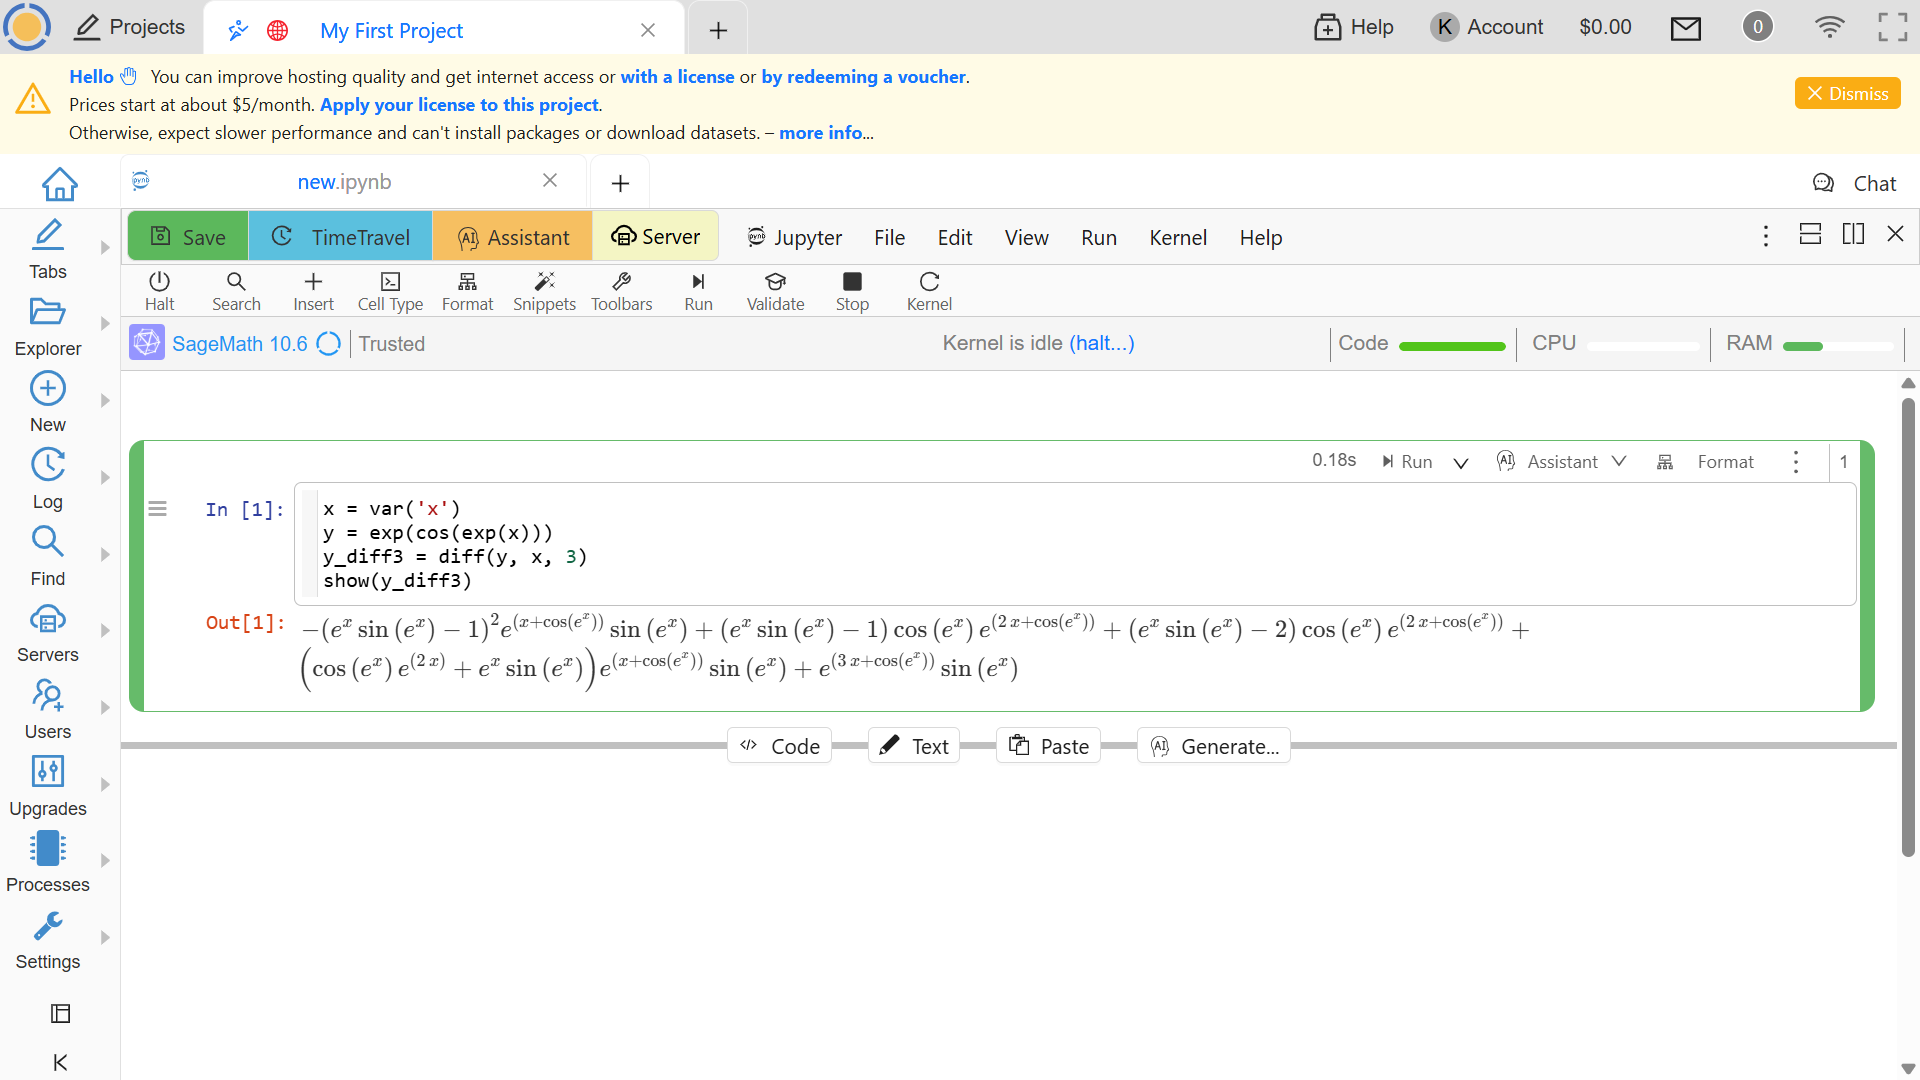
\includegraphics[width=0.7\linewidth]{images/screenshot004}
	\caption{Giao diện SageMath Notebook trên nền tảng trực tuyến CoCalc}
	\label{fig:screenshot004}
\end{figure}

\textbf{Hướng dẫn sử dụng CoCalc:}
\begin{itemize}
	\item Truy cập trang web: \url{https://cocalc.com}
	\item Đăng ký tài khoản hoặc sử dụng tài khoản Google để đăng nhập.
	\item Tạo một dự án mới (Project) và chọn môi trường SageMath.
	\item Tạo một file mới có phần mở rộng \texttt{.sagews} hoặc \texttt{.ipynb} để bắt đầu viết mã SageMath.
\end{itemize}

\textbf{Ưu điểm:}
\begin{itemize}
	\item Trực tiếp trên trình duyệt, không cần cài đặt.
	\item Hỗ trợ cộng tác và chia sẻ với người khác.
	\item Chạy được các notebook Jupyter có tích hợp SageMath.
\end{itemize}

\textbf{Nhược điểm:}
\begin{itemize}
	\item Phiên bản miễn phí có giới hạn tài nguyên.
	\item Cần kết nối internet ổn định.
\end{itemize}

\subsection{Binder - Chạy Notebook SageMath từ GitHub}

Binder là một dịch vụ trực tuyến cho phép chạy các notebook từ GitHub mà không cần cài đặt. Đây là giải pháp hiệu quả cho việc trình bày các đồ án và chia sẻ với giảng viên.
\begin{figure}[H]
	\centering
	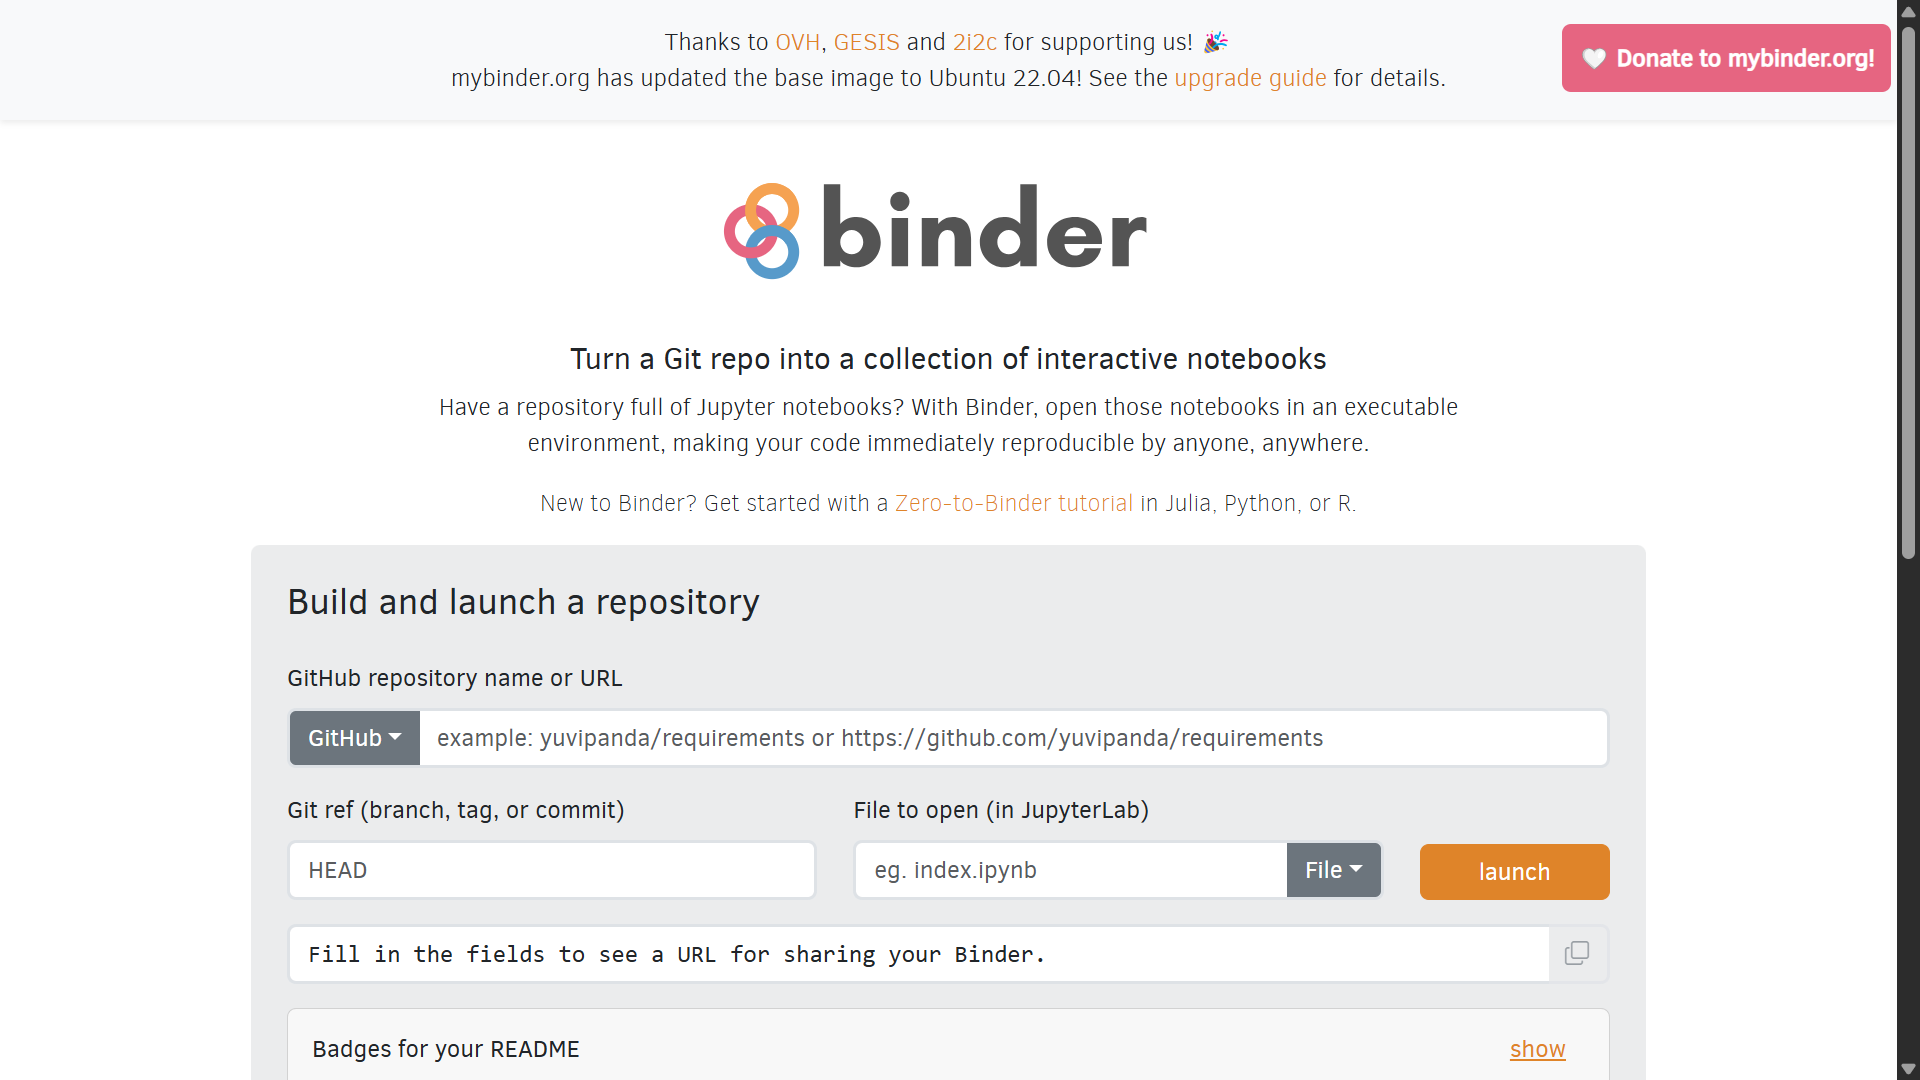
\includegraphics[width=0.7\linewidth]{images/screenshot003}
	\caption{Giao diện nền tảng Binder}
	\label{fig:screenshot003}
\end{figure}

\textbf{Hướng dẫn sử dụng Binder:}
\begin{itemize}
	\item Truy cập trang web: \url{https://mybinder.org}
	\item Nhập đường dẫn đến kho GitHub chứa file notebook.
	\item Chọn kernel SageMath nếu có, nhấn \texttt{Launch} để bắt đầu.
	\item Notebook sẽ được tải lên máy chủ và có thể chạy trực tuyến.
\end{itemize}

\textbf{Ưu điểm:}
\begin{itemize}
	\item Không cần đăng ký tài khoản.
	\item Dễ dàng chia sẻ với đường dẫn \textit{(link)} công khai.
\end{itemize}

\textbf{Nhược điểm:}
\begin{itemize}
	\item Khởi động lâu nếu dự án có nhiều thư viện.
	\item Không lưu lại trạng thái làm việc sau khi ngắt kết nối.
\end{itemize}

\subsection{Sage Cell - Tính toán nhanh với SageMath}

Sage Cell là công cụ trực tuyến cho phép thực thi các đoạn mã SageMath nhỏ mà không cần cài đặt.
\begin{figure}[H]
	\centering
	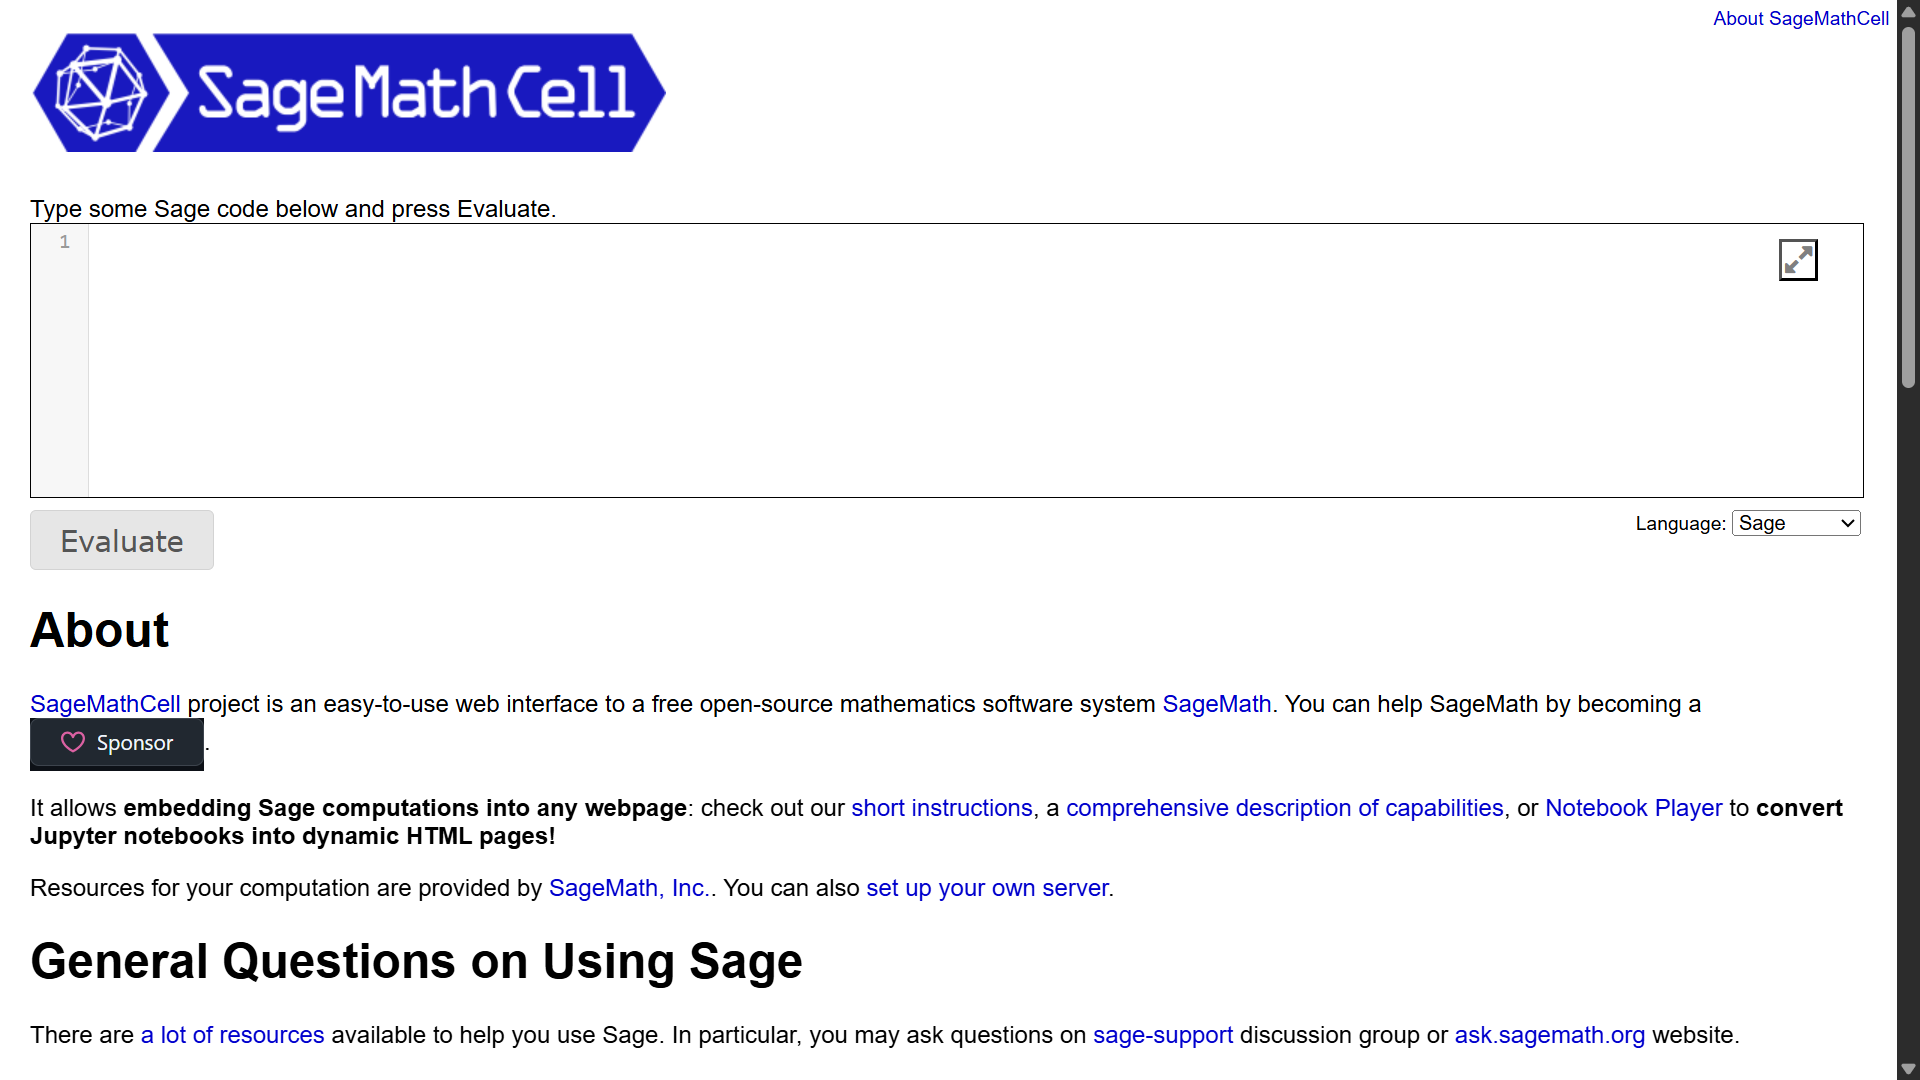
\includegraphics[width=0.7\linewidth]{images/screenshot002}
	\caption{Giao diện trang web Sage Cell}
	\label{fig:screenshot002}
\end{figure}

\textbf{Hướng dẫn sử dụng Sage Cell:}
\begin{itemize}
	\item Truy cập trang web: \url{https://sagecell.sagemath.org}
	\item Nhập mã SageMath vào ô nhập liệu.
	\item Nhấn \texttt{Evaluate} để xem kết quả.
\end{itemize}

\textbf{Ưu điểm:}
\begin{itemize}
	\item Nhanh chóng, không cần đăng nhập.
	\item Thích hợp cho các tính toán nhỏ.
\end{itemize}

\textbf{Nhược điểm:}
\begin{itemize}
	\item Không phù hợp với các dự án lớn hoặc tính toán phức tạp.
	\item Không có khả năng lưu trữ và cộng tác.
\end{itemize}

\subsection{So sánh các nền tảng trực tuyến}

\begin{table}[H]
	\centering
	\begin{tabular}{|c|c|c|c|}
		\hline
		\textbf{Nền tảng} & \textbf{Tính năng} & \textbf{Ưu điểm} & \textbf{Nhược điểm} \\
		\hline
		CoCalc & Tương tác mạnh mẽ & Hỗ trợ nhiều công cụ & Cần đăng ký tài khoản \\
		\hline
		Binder & Chạy từ GitHub & Dễ chia sẻ & Khởi động chậm \\
		\hline
		Sage Cell & Thực thi mã nhanh & Không cần đăng nhập & Chỉ tính toán nhỏ \\
		\hline
	\end{tabular}
	\caption{So sánh các nền tảng trực tuyến sử dụng SageMath}
\end{table}

\section{Giao diện và cách sử dụng cơ bản}

Sau khi cài đặt, người dùng có thể sử dụng SageMath theo các cách sau:

\begin{itemize}
	\item Giao diện dòng lệnh (CLI): khởi động bằng lệnh \texttt{sage}.
	\item Giao diện notebook (Jupyter): chạy lệnh \texttt{sage -n jupyter}.
	\item Giao diện đồ họa qua CoCalc nếu dùng trực tuyến.
\end{itemize}

\subsection*{Ví dụ cơ bản}

\begin{lstlisting}
	# Tinh tong 1 + 2 + ... + 100
	sum(i for i in (1..100))
	
	# Giai thua cua 10
	factorial(10)
	
	# Dao ham cua ham so
	f(x) = x^3 + x^2
	diff(f(x), x)
	
	# Ve do thi
	plot(sin(x), (x, -2*pi, 2*pi))
\end{lstlisting}

Sage hỗ trợ gần như toàn bộ các phép toán cơ bản đến nâng cao, cho phép nhập công thức trực tiếp theo cú pháp giống toán học thông thường.

